\documentclass[10pt,a4paper]{article}
\usepackage{lmodern}
\usepackage{amssymb,amsmath}
\usepackage{ifxetex,ifluatex}
\usepackage{fixltx2e} % provides \textsubscript
\ifnum 0\ifxetex 1\fi\ifluatex 1\fi=0 % if pdftex
  \usepackage[T1]{fontenc}
  \usepackage[utf8]{inputenc}
\else % if luatex or xelatex
  \ifxetex
    \usepackage{mathspec}
    \usepackage{xltxtra,xunicode}
  \else
    \usepackage{fontspec}
  \fi
  \defaultfontfeatures{Mapping=tex-text,Scale=MatchLowercase}
  \newcommand{\euro}{€}
\fi
% use upquote if available, for straight quotes in verbatim environments
\IfFileExists{upquote.sty}{\usepackage{upquote}}{}
% use microtype if available
\IfFileExists{microtype.sty}{%
\usepackage{microtype}
\UseMicrotypeSet[protrusion]{basicmath} % disable protrusion for tt fonts
}{}
\usepackage{color}
\usepackage{fancyvrb}
\newcommand{\VerbBar}{|}
\newcommand{\VERB}{\Verb[commandchars=\\\{\}]}
\DefineVerbatimEnvironment{Highlighting}{Verbatim}{commandchars=\\\{\}}
% Add ',fontsize=\small' for more characters per line
\usepackage{framed}
\definecolor{shadecolor}{RGB}{248,248,248}
\newenvironment{Shaded}{\begin{snugshade}}{\end{snugshade}}
\newcommand{\AlertTok}[1]{\textcolor[rgb]{0.94,0.16,0.16}{#1}}
\newcommand{\AnnotationTok}[1]{\textcolor[rgb]{0.56,0.35,0.01}{\textbf{\textit{#1}}}}
\newcommand{\AttributeTok}[1]{\textcolor[rgb]{0.77,0.63,0.00}{#1}}
\newcommand{\BaseNTok}[1]{\textcolor[rgb]{0.00,0.00,0.81}{#1}}
\newcommand{\BuiltInTok}[1]{#1}
\newcommand{\CharTok}[1]{\textcolor[rgb]{0.31,0.60,0.02}{#1}}
\newcommand{\CommentTok}[1]{\textcolor[rgb]{0.56,0.35,0.01}{\textit{#1}}}
\newcommand{\CommentVarTok}[1]{\textcolor[rgb]{0.56,0.35,0.01}{\textbf{\textit{#1}}}}
\newcommand{\ConstantTok}[1]{\textcolor[rgb]{0.00,0.00,0.00}{#1}}
\newcommand{\ControlFlowTok}[1]{\textcolor[rgb]{0.13,0.29,0.53}{\textbf{#1}}}
\newcommand{\DataTypeTok}[1]{\textcolor[rgb]{0.13,0.29,0.53}{#1}}
\newcommand{\DecValTok}[1]{\textcolor[rgb]{0.00,0.00,0.81}{#1}}
\newcommand{\DocumentationTok}[1]{\textcolor[rgb]{0.56,0.35,0.01}{\textbf{\textit{#1}}}}
\newcommand{\ErrorTok}[1]{\textcolor[rgb]{0.64,0.00,0.00}{\textbf{#1}}}
\newcommand{\ExtensionTok}[1]{#1}
\newcommand{\FloatTok}[1]{\textcolor[rgb]{0.00,0.00,0.81}{#1}}
\newcommand{\FunctionTok}[1]{\textcolor[rgb]{0.00,0.00,0.00}{#1}}
\newcommand{\ImportTok}[1]{#1}
\newcommand{\InformationTok}[1]{\textcolor[rgb]{0.56,0.35,0.01}{\textbf{\textit{#1}}}}
\newcommand{\KeywordTok}[1]{\textcolor[rgb]{0.13,0.29,0.53}{\textbf{#1}}}
\newcommand{\NormalTok}[1]{#1}
\newcommand{\OperatorTok}[1]{\textcolor[rgb]{0.81,0.36,0.00}{\textbf{#1}}}
\newcommand{\OtherTok}[1]{\textcolor[rgb]{0.56,0.35,0.01}{#1}}
\newcommand{\PreprocessorTok}[1]{\textcolor[rgb]{0.56,0.35,0.01}{\textit{#1}}}
\newcommand{\RegionMarkerTok}[1]{#1}
\newcommand{\SpecialCharTok}[1]{\textcolor[rgb]{0.00,0.00,0.00}{#1}}
\newcommand{\SpecialStringTok}[1]{\textcolor[rgb]{0.31,0.60,0.02}{#1}}
\newcommand{\StringTok}[1]{\textcolor[rgb]{0.31,0.60,0.02}{#1}}
\newcommand{\VariableTok}[1]{\textcolor[rgb]{0.00,0.00,0.00}{#1}}
\newcommand{\VerbatimStringTok}[1]{\textcolor[rgb]{0.31,0.60,0.02}{#1}}
\newcommand{\WarningTok}[1]{\textcolor[rgb]{0.56,0.35,0.01}{\textbf{\textit{#1}}}}
\usepackage{longtable,booktabs}
\ifxetex
  \usepackage[setpagesize=false, % page size defined by xetex
              unicode=false, % unicode breaks when used with xetex
              xetex]{hyperref}
\else
  \usepackage[unicode=true]{hyperref}
\fi
\hypersetup{breaklinks=true,
            bookmarks=true,
            pdfauthor={},
            pdftitle={titre non affiche},
            colorlinks=true,
            citecolor=blue,
            urlcolor=blue,
            linkcolor=magenta,
            pdfborder={0 0 0}}
\urlstyle{same}  % don't use monospace font for urls
\setlength{\parindent}{0pt}
\setlength{\parskip}{6pt plus 2pt minus 1pt}
\setlength{\emergencystretch}{3em}  % prevent overfull lines
\setcounter{secnumdepth}{5}

\providecommand{\tightlist}{%
  %\setlength{\itemsep}{0pt}
  \setlength{\parskip}{0pt}
  }

%%% Use protect on footnotes to avoid problems with footnotes in titles
\let\rmarkdownfootnote\footnote%
\def\footnote{\protect\rmarkdownfootnote}


  \title{titre non affiche}
    \author{}
    \date{}
  
% Packages

\usepackage[utf8]{inputenc}
\usepackage{setspace}
%\usepackage[french]{babel} % Pour la traduction française
%\renewcommand\frenchtablename{\textsc{Tableau}} %renommer table en tableau
%\AtBeginDocument{\renewcommand{\abstractname}{Synthèse}} %titre abstract
\usepackage{mathptmx} %times roman {mathptmx} OU {newtxtext} 
\DeclareSymbolFont{calletters}{OMS}{cmsy}{m}{n}  %pour differencier mathcal et mathscr
\DeclareSymbolFontAlphabet{\mathcal}{calletters} %pour differencier mathcal et mathscr
\usepackage[hmargin=1.5cm,vmargin=1.5cm]{geometry} % marges
\usepackage{caption}
\usepackage{graphicx}
\usepackage{natbib}
\usepackage[dvipsnames]{xcolor}
\usepackage{fontawesome5}
\DeclareMathOperator{\arctanh}{arctanh}
\usepackage{amsfonts}
\usepackage{dsfont}
\usepackage{xspace}
\usepackage{enumitem}
\usepackage{pifont}
\usepackage{wrapfig}
\usepackage{textpos}
\usepackage{array}
\usepackage{amsmath}
\usepackage{mathrsfs}  
\usepackage{tcolorbox}
\usepackage{here} %positionner les images
\usepackage{colortbl} %colorer un tableau
\usepackage[normalem]{ulem} %sout

\usepackage{ntheorem}
\theoremstyle{break}
\newtheorem{theorem}{Théorème}[section]
\newtheorem{lemma}{Lemme}[section]
\newtheorem{proposition}{Propriété}[section]
\newtheorem{corollary}{Corollaire}[section]
\newenvironment{proof}{\textbf{Preuve}}{$\Box$}
\newtheorem{definition}{Définition}[section]
\newtheorem{example}{Exemple}[section]
\newtheorem{remark}{Remarque}[section]
\newtheorem{conjecture}{Hypothèse}[section]
\newtheorem{problem}{Problème}[section]
\newtheorem{algo}{Algorithme}[section]
\def\cP{{\mathcal{P}}} 
\def\cM{{\mathcal{M}}} 
\def\CC{{\mathcal{C}}} 
\def\NN{{\mathbb{N}}}
\def\RR{{\mathbb{RR}}}
\definecolor{rougeENSAE}{RGB}{188, 24, 39}

%\onehalfspacing 



% % Page de garde
% 
% \makeatletter
% \def\@maketitle{%
%   \clearpage
%  \thispagestyle{empty}
% 
% \begin{textblock*}{\textwidth}(-7cm,-3.5cm)
% \begin{center}
% \includegraphics[height=3cm]{img/900px-LOGO-ENSAE.png}
% \end{center}
% \end{textblock*}
% 
% \begin{minipage}{0.3\textwidth}
%   \begin{flushleft} \large
%     \textbf{ANTUNEZ Kim \vspace{8.75mm} }
%   \end{flushleft}
% \end{minipage}
% \begin{minipage}{0.6\textwidth}
%   \begin{flushright} 
%   \large{
%     \textbf{ENSAE 2\up{ème} année\\}
%   }     
%   \small
%     \textbf{ 
%         \textit{Stage d'application\\
%         Année scolaire 2019 - 2020}
%     }
%   \end{flushright}
% \end{minipage}
% 
% \vspace*{2cm}
% 
% \begin{center}
%     \fbox{\parbox{0.9\textwidth}{
%         \begin{huge}\begin{center}
%             \textbf{Échantillonnage spatial déterminantal}\\
%         \end{center}\end{huge}}}
% \end{center}
% 
% \vfill
% 
% \begin{center}
% \includegraphics[width=0.6\linewidth]{img/markdown-figPG-1}
% \end{center}
% 
% \vfill
%     
% \begin{minipage}{0.4\textwidth}
%     \begin{flushleft} \large 
%     \textbf{Direction générale de l'Insee\\
%         Montrouge, France
%     }
%   \end{flushleft}
% \end{minipage} 
% \begin{minipage}{0.6\textwidth}
%   \begin{flushright} \large
%     \textbf{
%         Maître de stage : Vincent \textsc{Loonis}\\
%         08/06/2020 - 14/08/2020
%     }
%   \end{flushright}
% \end{minipage}    
% 
% \vspace*{1cm}
% 
% 
% \textcolor{rougeENSAE}{\rule{10mm}{1.5mm}}
% 
% \scriptsize
% \textbf{ENSAE Paris}\newline TSA 26644
% \rightline{\href{www.ensae.fr}{\textcolor{rougeENSAE}{\textbf{www.ensae.fr}}}$\quad \qquad \qquad$}
% Service des relations entreprises et des stages\newline
% 5, avenue Henry Le Chatelier -- 91764 PALAISEAU CEDEX -- FRANCE -- Tél : +33 (0)1 70 26 67 39 -- Courriel : stage\symbol{64}ensae.fr
% 
% \normalsize
% 
% \clearpage
% \setcounter{page}{1} %ne pas numéroter le sommaire: mettre 0
% \onehalfspacing
% 
% }
% 
% \makeatother% cinsérer page de garde

% Environnement colonnes

\newenvironment{cols}[1][]{}{}

\newenvironment{col}[1]{\begin{minipage}{#1}\ignorespaces}{%
\end{minipage}
\ifhmode\unskip\fi
\aftergroup\useignorespacesandallpars}

\def\useignorespacesandallpars#1\ignorespaces\fi{%
#1\fi\ignorespacesandallpars}

\makeatletter
\def\ignorespacesandallpars{%
  \@ifnextchar\par
    {\expandafter\ignorespacesandallpars\@gobble}%
    {}%
}
\makeatother
\usepackage{subfig}


\usepackage[tikz]{bclogo}
\newcounter{comptEncadre}
\renewcommand\thecomptEncadre{%\thesection.
\arabic{comptEncadre}}
\definecolor{processblue}{cmyk}{0.96,0,0,0}
\newenvironment{encadre}[2][false]{\refstepcounter{comptEncadre}
      %\addcontentsline{exp}{encadres}{\protect\numberline{\thecomptEncadre}#1}%
\begin{bclogo}[couleur=processblue!5,arrondi=0.1,
logo=\bcloupe,barre=none,couleurBord=blue!60!green,nobreak = #1]{ {\sc \textbf{Encadré \thecomptEncadre}} -  #2}
\smallskip
}{\end{bclogo}}


% nouvelle page de titre Kim
\usepackage{titling}
\setlength{\droptitle}{-8em}
\usepackage{lipsum}
\title{\textbf{\emph{PageRank} : de l'algorithme classique aux calculs distribués} \medskip \\ \large \emph{Kim ANTUNEZ, Isabelle BERNARD (année 2020-2021)}}
\author{}


\renewcommand\maketitlehookc{\vspace{-10ex}}
% nouvelle page de titre Kim

%espaces entre sections Kim
\usepackage{titlesec}
\titlespacing*{\section}
{0pt}{1.5ex plus 1ex minus .2ex}{0.3ex plus .2ex}
\titlespacing*{\subsection}
{0pt}{1.5ex plus 1ex minus .2ex}{0.3ex plus .2ex}
%espaces entre sections Kim


\begin{document}

\maketitle


\vspace{-15truemm}

\hypertarget{introduction}{%
\section{Introduction}\label{introduction}}

\emph{PageRank} est un algorithme, parmi d'autres, qui mesure la popularité d'une page web. Il fonctionne en classant les pages du Web en fonction de leur popularité (voir description détaillée dans les parties qui suivent).

Il a été inventé par Larry Page (\cite{Brin}), cofondateur de Google, et est utilisé par le moteur de recherche de l'entreprise. Il s'agit d'une marque déposée dont le premier brevet a été déposé en 1997. Jusqu'en 2016, les internautes pouvaient obtenir une approximation du classement de chaque page mais, depuis, Google ne fournit plus cette valeur.

\hypertarget{principe-recherchuxe9-par-pagerank}{%
\subsection{\texorpdfstring{Principe recherché par \emph{PageRank}}{Principe recherché par PageRank}}\label{principe-recherchuxe9-par-pagerank}}

\begin{figure}[htp]
\begin{center}
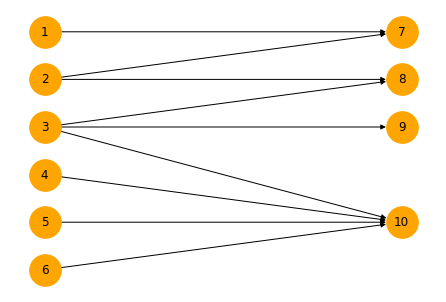
\includegraphics[width=0.4\textwidth]{img/DocPageRank_files/DocPageRank_2_0.png}
\end{center}
\captionsetup{margin=0cm,format=hang,justification=justified}
\caption{Exemple de graphe}\label{fig:fig0}
\end{figure}

La modélisation adoptée utilise la théorie des graphes. Le web est un \textbf{graphe orienté} \(G\) contient \(N\) \textbf{noeuds} (dans la figure~\ref{fig:fig0}, \(N = 10\) pages) reliés par des \textbf{liens} orientés (hyperliens). Un \textbf{degré entrant} (\emph{in-degree}) d'une page correspond aux nombre d'hyperliens qui pointent sur elle et le \textbf{degré sortant} (\emph{out-degree}) le nombre d'hyperliens vers lesquels elle pointe.

Si l'on veut faire une première vulgarisation de l'algorithme, on peut dire que \emph{PageRank} cherche à respecter les propriétés suivantes~:

\begin{enumerate}
\def\labelenumi{\arabic{enumi}.}
\tightlist
\item
  \textbf{Popularité absolue} : plus le nombre de pages citant une page est grande, plus sa popularité doit être élevée.
\end{enumerate}

\emph{Exemple : Dans la figure \ref{fig:fig0}, le noeud \(10\) est particulièrement populaire car 4 noeuds (les \(3\), \(4\), \(5\) et \(6\)) pointent vers lui.}

\begin{enumerate}
\def\labelenumi{\arabic{enumi}.}
\setcounter{enumi}{1}
\tightlist
\item
  \textbf{Popularité relative} : quand deux pages sont citées le même nombre de fois, c'est la page qui a été le plus cité en proportion par ses voisins qui doit être la plus populaire.
\end{enumerate}

\emph{Exemple : On cherche à distinguer la popularité des noeuds \(7\) et \(8\) qui ont chacun deux noeuds qui pointent vers eux. On considère que le noeud \(7\) est plus populaire car le noeud \(1\) popularise exclusivement ce noeud, alors que le noeud \(3\) popularise le noeud \(8\) dans une moindre mesure car il popularise 2 autres noeuds (\(9\) et \(10\)).}

\faArrowCircleRight{} \emph{PageRank} se rapproche d'une mesure de centralité sur le réseau du web. \textbf{Plus la page web a de chance d'être dans les premières positions lors d'une recherche sur internet, plus le \emph{PageRank} sera élevé}. Son principe est d'attribuer à chaque page un score proportionnel au nombre de fois que passerait par cette page un utilisateur parcourant le graphe du Web en cliquant aléatoirement, sur un des liens apparaissant sur chaque page. Une page a un \emph{PageRank} d'autant plus important qu'est grande la somme des \emph{PageRanks} des pages qui pointent vers elle.

\hypertarget{algorithme-de-pagerank}{%
\subsection{\texorpdfstring{Algorithme de \emph{PageRank}}{Algorithme de PageRank}}\label{algorithme-de-pagerank}}

La valeur (ou rang) \emph{PageRank} d'une page \(p\) (\(r(p)\)) dépend des valeurs \emph{PageRank} de chacune des pages \(q\) qui pointent vers la page \(p\) (\(q \rightarrow p\)) divisées par le nombre de noeuds auxquels fait référence la page \(q\) (\(d(q)\) = degré sortant) :

\begin{equation} \label{eq:eq1}
r(p)=\sum_{ q \rightarrow p}\frac{r(q)}{d(q)}
\end{equation}

L'équation \ref{eq:eq1} peut être réécrite sous forme matricielle \(\vec{r} = L \vec{r}\) où le vecteur \(\vec{r}\) est le vecteurs des valeurs PageRank des \(N\) pages et la matrice \(L\) est telle que \(L[q, p] = \frac{1}{d(q)}\) s'il y a un lien qui relit le noeud \(q\) au noeud \(p\) et qui vaut 0 sinon.

Le programme peut être résolu par l'algorithme de la puissance itérée (\emph{power iteration method}) qui repose sur le théorème de Perron-Frobenius et est dédié à la recherche de valeurs et vecteurs propres. Cet algorithme est utilisé dans le cas de PageRank en raison de la grande taille de la matrice qui encourage à utiliser la matrice au travers de produits, mais sa vitesse de convergence (convergence qui d'ailleurs n'est pas garantie) est assez lente. On stoppe donc l'algorithme après un certain nombre d'itérations ou si la norme \(L^1\) de l'écart des valeurs \emph{PageRank} entre 2 itérations est inférieure à un certain seuil de tolérance qui dépend de \(N\).

\hypertarget{approximation-locale-de-pagerank}{%
\subsection{\texorpdfstring{Approximation locale de \emph{PageRank}}{Approximation locale de PageRank}}\label{approximation-locale-de-pagerank}}

La très grande taille de ce graphe et son évolution rendent coûteuses en opérations le calcul d'un \emph{PageRank} pour une nouvelle page. C'est pourquoi des \textbf{algorithmes d'approximation} existent.

L'approximation locale de l'algorithme \emph{PageRank} que nous utilisons s'appuie sur l'article \cite{Chen}.

Il s'agit d'approximer le vecteur des rangs de l'ensemble des pages en faisant un calcul itératif (marche aléatoire). Après avoir initialisé un rang de \(\frac{1}{N}\) pour toutes les pages, on met à jour le vecteur de rangs de la manière suivante où \(i\) correspond au numéro de l'itération :

\begin{equation} \label{eq:eq2}
r^{i+1}(p)=\sum_{ q \rightarrow p}\frac{r^{i}(q)}{d(q)}
\end{equation}

Cependant, dans cette formulation, si un noeud \(p\) n'a pas de degré sortant \(q\), c'est-à-dire qu'il ne fait référence à aucune page (\emph{dangling node}), son rang n'est pas mis à jour dans l'algorithme à l'itération suivante, ce qui entraîne une perte de la valeur totale du \emph{PageRank}. Une solution serait de nettoyer itérativement le graphe en enlevant les pages sans hyperliens. Mais, même en procédant ainsi, le graphe peut toujours contenir des groupes de pages très peu connectés entre eux qui posent le même problème. C'est pourquoi on introduit un facteur d'amortissement \(\alpha\) (par exemple \(\alpha = 0,85\), \emph{teleportation factor}). Tout marche comme si on réalise l'algorithme précédent (c'est-à-dire on choisit aléatoirement un degré sortant du noeud considéré) avec une probabilité \(\alpha\) et on choisit un noeud au hasard avec la probabilité \(1-\alpha\) (\emph{damping factor}) :

\begin{equation} \label{eq:eq3}
r^{i+1}(p)=\frac{1-\alpha}{N}+\alpha \sum_{ q \rightarrow p}\frac{r^{i}(q)}{d(q)}
\end{equation}

Le paramètre \(\alpha\) est fixé par le \emph{data-scientist}. Ainsi, l'algorithme tel que nous l'avons décrit (y compris son initialisation) est \textbf{déterministe} : on obtient toujours le même résultat à nombre d'itération et \(\alpha\) fixés.

\hypertarget{approximation-locale-de-pagerank-avec-lapproche-mapreduce-avec-spark}{%
\subsection{\texorpdfstring{Approximation locale de \emph{PageRank} avec l'approche MapReduce avec Spark}{Approximation locale de PageRank avec l'approche MapReduce avec Spark}}\label{approximation-locale-de-pagerank-avec-lapproche-mapreduce-avec-spark}}

Comme évoqué en cours d'ELTDM, \textbf{MapReduce}, inventé également par Google, permet d'effectuer des calculs parallèles, et souvent distribués, de données potentiellement très volumineuses, en les distribuant dans un cluster de machines.

Nous avons vu que l'algorithme \emph{PageRank} est récursif, itératif, et dépend d'une structure de millions d'hyperliens. Le fait de l'implémenter sur une unique machine dont la mémoire doit disposer de l'ensemble du graphe le rend difficilement « scalable ». C'est pourquoi l'utilisation d'une structure en map-reduce se justifie largement ici.

\textbf{Spark} est un framework open source qui permet de faire le calcul distribué dont nous avons besoin. Il réalise une lecture des données au niveau du cluster (grappe de serveurs sur un réseau), effectue toutes les opérations d'analyse nécessaires, puis écrit les résultats à ce même niveau.

Spark ne manipule pas des données classiques mais des \textbf{R}esilient \textbf{D}istributed \textbf{D}ataset ou \textbf{RDD}, une collection de données calculée et conservée en mémoire vive. Ce sont des lignes de données, non modifiables (toute modification implique la création d'un nouveau RDD), qui ne peuvent pas être cassées (il faut parcourir le fichier en entier, il n'y a pas d'index) et qui sont distribuées dans un ordre imprévisible dans les différents clusters.

Grâce à la librairie python \texttt{pyspark} nous avons pu nous initier à cette technologie en l'utilisant sur nos PC \textbf{en local}.

\hypertarget{version-simplifiuxe9e}{%
\subsubsection{Version simplifiée}\label{version-simplifiuxe9e}}

Nous l'avons vu, l'idée générale de \emph{PageRank} est de \textbf{répandre} les masses de probabilités au fil de chaque flux d'\textbf{hyperliens sortants}. A la fin de chaque itération, chaque noeud est résumé par une valeur \emph{PageRank} qui résume les fois où l'utilisateur navigant au hasard passe par la page (voir la figure \ref{fig:fig1} qui résume différentes itérations de l'algorithme dans le cas simplificateur où \(\alpha = 1\)).

\newpage

\begin{figure}[htp]
\begin{center}
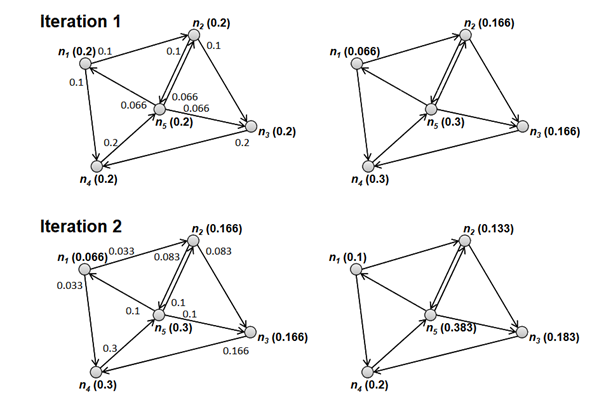
\includegraphics[width=0.6\textwidth]{img/img1.png}
\captionsetup{margin=0cm,format=hang,justification=justified}
\caption{Schéma de l'algorithme \emph{PageRank}}\label{fig:fig1}
%\vspace{-0.3cm}
\emph{Source : \cite{Lin}}
\end{center}
\end{figure}

L'implémentation MapReduce de PageRank est telle que chaque itération se décompose en 2 phases (cf.~figure \ref{fig:fig2}) :

\begin{enumerate}
\def\labelenumi{\arabic{enumi}.}
\tightlist
\item
  la phase « Map » : on sépare chaque noeud (page) associé à ses hyperliens
\item
  la phase « Reduce » : les contributions sont sommées pour tous les noeuds de destination
\end{enumerate}

\begin{figure}[htp]
\begin{center}
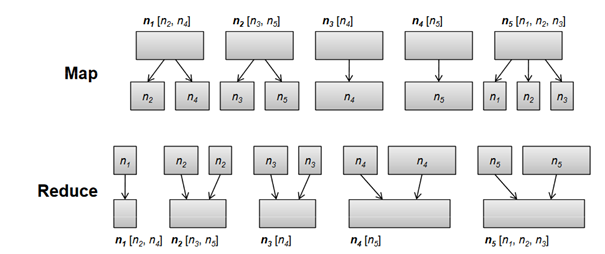
\includegraphics[width=0.6\textwidth]{img/img2.png}
\captionsetup{margin=0cm,format=hang,justification=justified}
\caption{Schéma de l'algorithme \emph{PageRank} avec l'approche \emph{MapReduce}}\label{fig:fig2}
%\vspace{-0.3cm}
\emph{Source : \cite{Lin}}
\end{center}
\end{figure}

Cela se traduit algorithmiquement par le pseudo-code suivant :

\begin{verbatim}
    classMapper
        method Map(nid n,node N)
        p<- N.PageRank/|N.AdjacencyList|
        Emit(nidn,N) #Pass along graph structure
        for all nodeid m in N.AdjacencyList do
            Emit(nidm,p) #Pass PageRank mass to neighbors

    classReducer
        method Reduce(nid m,[p1,p2,...])
        M <- empty set
        for all p in counts [p1,p2,...] do
            if IsNode(p) then
                M <- p #Recover graph structure
            else
                s <- s+p #Sum incoming PageRank contributions
        M.PageRank <- s
        Emit(nid m,node M)
\end{verbatim}

\emph{Source : Lin, Dyer 2010}

\hypertarget{introduction-du-facteur-alpha}{%
\subsubsection{\texorpdfstring{Introduction du facteur \(\alpha\)}{Introduction du facteur \textbackslash{}alpha}}\label{introduction-du-facteur-alpha}}

La modélisation se complique légèrement quand on considère le facteur \(\alpha\), on fait intervenir alors deux termes dans la somme de l'étape \emph{reduce}, comme modélisé dans l'équation \ref{eq:eq3}.

La modélisation se complique encore davantage en présence de \emph{dangling} nodes. En plus d'ajouter le facteur \(\alpha\), il s'agit également de redistribuer (faire un nouveau mapping sur tous les noeuds) la masse perdue à l'ensemble des noeuds du graphe de manière égale.

\textbf{\faArrowCircleRight{} Ici, nous simplifions légèrement le processus en supprimant les quelques \emph{dangling nodes} présents dans les données et nous nous concentrons sur l'implémentation des 3 méthodes évoquées plus haut :}

\textbf{1. L'algorithme de \emph{PageRank} global (\texttt{pagerank\_global})}

\textbf{2. Son approximation locale telle que décrite dans l'article \cite{Chen} (\texttt{pagerank\_local})}

\textbf{3. La version parallélisée de l'approximation locale en utilisant les calculs distribués grâce à Spark (\texttt{pagerank\_local\_spark})}

\hypertarget{application-calcul-distribuuxe9-vs-non-distribuuxe9}{%
\section{Application : calcul distribué VS non-distribué}\label{application-calcul-distribuuxe9-vs-non-distribuuxe9}}

La base de données utilisée provient de la \href{http://snap.stanford.edu/data/index.html}{librairie SNAP} de l'université de Stanford. Les données qui y sont mises à disposition l'ont été dans la plupart du temps dans des objectifs de recherche.

Il s'agit du fichier \texttt{web-Google}, mis à disposition par Google en 2002 lors d'un concours de programmeurs, dont les 875 713 noeuds représentent des pages webs et les 5 105 039 liens orientés représentent les hyperliens.

\begin{Shaded}
\begin{Highlighting}[]
\ImportTok{from}\NormalTok{ pyspark }\ImportTok{import}\NormalTok{ SparkContext, SparkConf}
\ImportTok{import}\NormalTok{ numpy }\ImportTok{as}\NormalTok{ np}
\ImportTok{import}\NormalTok{ pandas }\ImportTok{as}\NormalTok{ pd}
\ImportTok{import}\NormalTok{ random}
\ImportTok{import}\NormalTok{ networkx }\ImportTok{as}\NormalTok{ nx}
\ImportTok{import}\NormalTok{ matplotlib.pyplot }\ImportTok{as}\NormalTok{ plt}
\ImportTok{from}\NormalTok{ timeit }\ImportTok{import}\NormalTok{ default_timer}
\OperatorTok{%}\NormalTok{matplotlib inline}
\CommentTok{#%matplotlib notebook}
\ImportTok{from}\NormalTok{ operator }\ImportTok{import}\NormalTok{ add}
\end{Highlighting}
\end{Shaded}

\hypertarget{fonctions-utiles}{%
\subsection{Fonctions utiles}\label{fonctions-utiles}}

Divers

\begin{Shaded}
\begin{Highlighting}[]
\CommentTok{# Charger les données de réseaux, sélectionner le nombre de lignes à garder}
\CommentTok{# et enregistrer le fichier. }
\KeywordTok{def}\NormalTok{ sauver_donnees(nb_lignes}\OperatorTok{=}\DecValTok{60}\NormalTok{, fichier}\OperatorTok{=}\StringTok{"web-Google"}\NormalTok{):}
\NormalTok{    dfFile }\OperatorTok{=}\NormalTok{ pd.read_csv(}\StringTok{"data/}\SpecialCharTok{\{\}}\StringTok{.txt"}\NormalTok{.}\BuiltInTok{format}\NormalTok{(fichier), sep}\OperatorTok{=}\StringTok{'}\CharTok{\textbackslash{}t}\StringTok{'}\NormalTok{,}
\NormalTok{                             header}\OperatorTok{=}\DecValTok{3}\NormalTok{, nrows }\OperatorTok{=}\NormalTok{ nb_lignes)}
\NormalTok{    nodesList }\OperatorTok{=}\NormalTok{ dfFile[}\StringTok{'# FromNodeId'}\NormalTok{].unique()}
    \CommentTok{#enlever les donnees inutiles}
\NormalTok{    dfFile }\OperatorTok{=}\NormalTok{ dfFile[dfFile[}\StringTok{'ToNodeId'}\NormalTok{].isin(nodesList)] }
\NormalTok{    dfFile.to_csv(}\StringTok{"data/}\SpecialCharTok{\{\}\{\}}\StringTok{.txt"}\NormalTok{.}\BuiltInTok{format}\NormalTok{(fichier, nb_lignes), sep}\OperatorTok{=}\StringTok{' '}\NormalTok{,}
\NormalTok{                  header}\OperatorTok{=}\VariableTok{False}\NormalTok{, index}\OperatorTok{=}\VariableTok{False}\NormalTok{)}
    
\CommentTok{# Afficher les résultats de l'algorithme PageRank à l'utilisateur}
\KeywordTok{def}\NormalTok{ afficher_resultats_PR(resultat):}
\NormalTok{    duration }\OperatorTok{=}\NormalTok{ resultat[}\DecValTok{0}\NormalTok{]}
\NormalTok{    ranks }\OperatorTok{=}\NormalTok{ resultat[}\DecValTok{1}\NormalTok{]}
    \ControlFlowTok{for}\NormalTok{ key }\KeywordTok{in}\NormalTok{ ranks: }\CommentTok{# 3 chiffres significatifs}
\NormalTok{        ranks[key] }\OperatorTok{=} \BuiltInTok{round}\NormalTok{(ranks[key], }\DecValTok{3}\NormalTok{) }
    \BuiltInTok{print}\NormalTok{(}\SpecialStringTok{f'Le temps de calcul est de }\SpecialCharTok{\{}\BuiltInTok{round}\NormalTok{(duration,}\DecValTok{4}\NormalTok{)}\SpecialCharTok{\}}\SpecialStringTok{ secondes'}\NormalTok{)}
    \BuiltInTok{print}\NormalTok{(}\SpecialStringTok{f'La liste des noeuds et de leurs valeurs PageRank finales est'}\NormalTok{)}
    \BuiltInTok{print}\NormalTok{(ranks)}
    \BuiltInTok{print}\NormalTok{(}\StringTok{'}\CharTok{\textbackslash{}n}\StringTok{'}\NormalTok{)}
\end{Highlighting}
\end{Shaded}

Les différents algorithmes de PageRank (global, local non distribué et distribué)

\begin{Shaded}
\begin{Highlighting}[]
\KeywordTok{def}\NormalTok{ pagerank_global(G, alpha}\OperatorTok{=}\DecValTok{1}\NormalTok{, max_iter}\OperatorTok{=}\DecValTok{100}\NormalTok{, tol}\OperatorTok{=}\DecValTok{10000000000000000}\NormalTok{): }
  
    \CommentTok{"""Retourne : un dictionnaire de noeuds dont les valeurs correspondent}
\CommentTok{     aux PageRank ainsi que le temps de calcul de l'algorithme}
\CommentTok{      }
\CommentTok{    Paramètres}
\CommentTok{    ---------- }
\CommentTok{    -G : graph (de type NetworkX) }
\CommentTok{    -alpha : paramètre d'amortissement (1 par défaut) }
\CommentTok{    -max_iter : nombre maximum d'itération dans la recherche de valeurs propres. }
\CommentTok{    -tol : erreur de tolérence acceptée pour la convergence}
\CommentTok{    de la méthode de recherche des valeurs propres. }
\CommentTok{     }
\CommentTok{    """}
    
\NormalTok{    start }\OperatorTok{=}\NormalTok{ default_timer()}
    
    \CommentTok{# Créer une copie sous forme de graphique droit-stochastique (pour chaque noeud, }
    \CommentTok{# la somme des poids des liens sortant vaut 1)    }
\NormalTok{    W }\OperatorTok{=}\NormalTok{ nx.stochastic_graph(G, weight}\OperatorTok{=}\VariableTok{None}\NormalTok{)}
\NormalTok{    N }\OperatorTok{=}\NormalTok{ W.number_of_nodes() }
  
    \CommentTok{# Initialisation à 1/N }
\NormalTok{    x }\OperatorTok{=} \BuiltInTok{dict}\NormalTok{.fromkeys(W, }\FloatTok{1.0} \OperatorTok{/}\NormalTok{ N) }
\NormalTok{    p }\OperatorTok{=} \BuiltInTok{dict}\NormalTok{.fromkeys(W, }\FloatTok{1.0} \OperatorTok{/}\NormalTok{ N)}
\NormalTok{    dangling_weights }\OperatorTok{=}\NormalTok{ x }
\NormalTok{    dangling_nodes }\OperatorTok{=}\NormalTok{ [n }\ControlFlowTok{for}\NormalTok{ n }\KeywordTok{in}\NormalTok{ W }\ControlFlowTok{if}\NormalTok{ W.out_degree(n, weight}\OperatorTok{=}\VariableTok{None}\NormalTok{) }\OperatorTok{==} \FloatTok{0.0}\NormalTok{] }
    
    \CommentTok{#algorithme de la puissance itérée}
    \ControlFlowTok{for}\NormalTok{ _ }\KeywordTok{in} \BuiltInTok{range}\NormalTok{(max_iter): }
\NormalTok{        xlast }\OperatorTok{=}\NormalTok{ x }
\NormalTok{        x }\OperatorTok{=} \BuiltInTok{dict}\NormalTok{.fromkeys(xlast.keys(), }\DecValTok{0}\NormalTok{)}
\NormalTok{        danglesum }\OperatorTok{=}\NormalTok{ alpha }\OperatorTok{*} \BuiltInTok{sum}\NormalTok{(xlast[n] }\ControlFlowTok{for}\NormalTok{ n }\KeywordTok{in}\NormalTok{ dangling_nodes) }
        \ControlFlowTok{for}\NormalTok{ n }\KeywordTok{in}\NormalTok{ x: }
  
            \CommentTok{# multiplication à gauche x^T=xlast^T*W }
            \ControlFlowTok{for}\NormalTok{ nbr }\KeywordTok{in}\NormalTok{ W[n]: }
\NormalTok{                x[nbr] }\OperatorTok{+=}\NormalTok{ alpha }\OperatorTok{*}\NormalTok{ xlast[n] }\OperatorTok{*}\NormalTok{ W[n][nbr][}\VariableTok{None}\NormalTok{] }
\NormalTok{            x[n] }\OperatorTok{+=}\NormalTok{ danglesum }\OperatorTok{*}\NormalTok{ dangling_weights[n] }\OperatorTok{+}\NormalTok{ (}\DecValTok{1}\OperatorTok{-}\NormalTok{alpha) }\OperatorTok{*}\NormalTok{ p[n] }
          
        \CommentTok{# vérifier la convergence L1}
\NormalTok{        err }\OperatorTok{=} \BuiltInTok{sum}\NormalTok{([}\BuiltInTok{abs}\NormalTok{(x[n] }\OperatorTok{-}\NormalTok{ xlast[n]) }\ControlFlowTok{for}\NormalTok{ n }\KeywordTok{in}\NormalTok{ x]) }
        \ControlFlowTok{if}\NormalTok{ err }\OperatorTok{<}\NormalTok{ N}\OperatorTok{*}\NormalTok{tol:}
\NormalTok{            duration }\OperatorTok{=}\NormalTok{ default_timer() }\OperatorTok{-}\NormalTok{ start}
\NormalTok{            retour }\OperatorTok{=}\NormalTok{ (duration, x)}
            \ControlFlowTok{return}\NormalTok{ retour}
    \ControlFlowTok{raise}\NormalTok{ NetworkXError(}\StringTok{'pagerank: erreur de convergence au bout '}
                        \StringTok{'de }\SpecialCharTok\NormalTok{ max_iter) }
\end{Highlighting}
\end{Shaded}

\begin{Shaded}
\begin{Highlighting}[]
\KeywordTok{def}\NormalTok{ pagerank_local(G, alpha}\OperatorTok{=}\DecValTok{1}\NormalTok{, max_iter}\OperatorTok{=}\DecValTok{10}\NormalTok{,}
\NormalTok{                   only_timer}\OperatorTok{=}\VariableTok{False}\NormalTok{, timer_mapreduce}\OperatorTok{=}\VariableTok{True}\NormalTok{):  }

    \CommentTok{"""Retourne : un dictionnaire de noeuds dont les valeurs correspondent}
\CommentTok{     aux PageRank ainsi que le temps de calcul de l'algorithme}
\CommentTok{      }
\CommentTok{    Paramètres}
\CommentTok{    ---------- }
\CommentTok{    -G : graph (de type NetworkX) }
\CommentTok{    -alpha : paramètre d'amortissement (1 par défaut) }
\CommentTok{    -max_iter : nombre maximum d'itération dans la recherche de valeurs propres. }
\CommentTok{    - only_timer : si vaut True, ne retourne que le temps de calcul, sinon retourne }
\CommentTok{    aussi la valeur des rangs à la dernière itération }
\CommentTok{    - timer_mapreduce : si vaut True, le timer calcul l'efficacité de calcul qui peut}
\CommentTok{    être distribuée (map-reduce). si vaut False, le timer calcul le temps}
\CommentTok{    d'initialisation}
\CommentTok{    }
\CommentTok{    """}
    
    \CommentTok{### Initialisation}
    \ControlFlowTok{if} \KeywordTok{not}\NormalTok{ timer_mapreduce:}
\NormalTok{            start }\OperatorTok{=}\NormalTok{ default_timer()}
    \CommentTok{# Successors and Predecessors}
\NormalTok{    successors }\OperatorTok{=}\NormalTok{ \{node: }\BuiltInTok{list}\NormalTok{(G.successors(node)) }\ControlFlowTok{for}\NormalTok{ node }\KeywordTok{in} \BuiltInTok{list}\NormalTok{(G.nodes())\} }
\NormalTok{    predecessors }\OperatorTok{=}\NormalTok{ \{node: }\BuiltInTok{list}\NormalTok{(G.predecessors(node)) }\ControlFlowTok{for}\NormalTok{ node }\KeywordTok{in} \BuiltInTok{list}\NormalTok{(G.nodes())\}}
    \CommentTok{# Calcul du nombre total de noeuds (pages)}
\NormalTok{    N }\OperatorTok{=}\NormalTok{ G.number_of_nodes() }
    \CommentTok{# Initialisation chacun des rangs à 1/N}
\NormalTok{    ranks }\OperatorTok{=}\NormalTok{ \{node: }\FloatTok{1.0}\OperatorTok{/}\NormalTok{N }\ControlFlowTok{for}\NormalTok{ node }\KeywordTok{in} \BuiltInTok{list}\NormalTok{(G.nodes())\} }
    \ControlFlowTok{if} \KeywordTok{not}\NormalTok{ timer_mapreduce:}
\NormalTok{            duration }\OperatorTok{=}\NormalTok{ default_timer() }\OperatorTok{-}\NormalTok{ start}
    
    \CommentTok{# Lancer le chronomètre pour comparer partie non distribuée }
    \CommentTok{# avec la partie distribuée}
    \ControlFlowTok{if}\NormalTok{ timer_mapreduce:}
\NormalTok{            start }\OperatorTok{=}\NormalTok{ default_timer()}
    
    \ControlFlowTok{for}\NormalTok{ i }\KeywordTok{in} \BuiltInTok{range}\NormalTok{(max_iter):}
\NormalTok{        r_sur_d }\OperatorTok{=}\NormalTok{ \{node :(}\BuiltInTok{float}\NormalTok{(}\FloatTok{1.0}\OperatorTok{/}\NormalTok{N) }\ControlFlowTok{if} \BuiltInTok{len}\NormalTok{(successors[node])}\OperatorTok{==}\DecValTok{0}
          \ControlFlowTok{else} \BuiltInTok{float}\NormalTok{(ranks[node]}\OperatorTok{/}\BuiltInTok{len}\NormalTok{(successors[node]))) }\ControlFlowTok{for}\NormalTok{ node }\KeywordTok{in} \BuiltInTok{list}\NormalTok{(G.nodes())\}}
\NormalTok{        ranks_new }\OperatorTok{=}\NormalTok{ \{}
\NormalTok{            node: (}\DecValTok{1}\OperatorTok{-}\NormalTok{alpha)}\OperatorTok{/}\NormalTok{N }\OperatorTok{+}
\NormalTok{            alpha }\OperatorTok{*} \BuiltInTok{sum}\NormalTok{([r_sur_d[key] }\ControlFlowTok{for}\NormalTok{ key }\KeywordTok{in}\NormalTok{ predecessors[node]])}
            \ControlFlowTok{for}\NormalTok{ node }\KeywordTok{in} \BuiltInTok{list}\NormalTok{(G.nodes())}
\NormalTok{        \}}
        \CommentTok{#print(sum(ranks_new.values()))}
\NormalTok{        ranks }\OperatorTok{=}\NormalTok{ ranks_new}
    \ControlFlowTok{if}\NormalTok{ timer_mapreduce:}
\NormalTok{            duration }\OperatorTok{=}\NormalTok{ default_timer() }\OperatorTok{-}\NormalTok{ start}
    \ControlFlowTok{if}\NormalTok{ only_timer:}
\NormalTok{        retour}\OperatorTok{=}\NormalTok{duration}
    \ControlFlowTok{else}\NormalTok{:}
\NormalTok{        retour}\OperatorTok{=}\NormalTok{(duration, ranks)}
    \ControlFlowTok{return}\NormalTok{ retour}
\end{Highlighting}
\end{Shaded}

\begin{Shaded}
\begin{Highlighting}[]
\CommentTok{# Récupère un noeud entrant et son noeud sortant et les met dans une liste. }
\KeywordTok{def}\NormalTok{ ligne_vers_node(ligne):}
\NormalTok{    nodes }\OperatorTok{=}\NormalTok{ ligne.split(}\StringTok{' '}\NormalTok{) }
    \ControlFlowTok{return} \BuiltInTok{int}\NormalTok{(nodes[}\DecValTok{0}\NormalTok{]), }\BuiltInTok{int}\NormalTok{(nodes[}\DecValTok{1}\NormalTok{])}

\KeywordTok{def}\NormalTok{ pagerank_local_spark(RddDataBase,alpha}\OperatorTok{=}\DecValTok{1}\NormalTok{, max_iter}\OperatorTok{=}\DecValTok{10}\NormalTok{,}
\NormalTok{                         only_timer}\OperatorTok{=}\VariableTok{False}\NormalTok{,timer_mapreduce}\OperatorTok{=}\VariableTok{True}\NormalTok{): }

    \CommentTok{"""Retourne : un dictionnaire de noeuds dont les valeurs correspondent}
\CommentTok{     aux PageRank ainsi que le temps de calcul de l'algorithme}
\CommentTok{      }
\CommentTok{    Paramètres}
\CommentTok{    ---------- }
\CommentTok{    -RddDataBase : graph (de type RDD) }
\CommentTok{    -alpha : paramètre d'amortissement (1 par défaut) }
\CommentTok{    -max_iter : nombre maximum d'itération dans la recherche de valeurs propres. }
\CommentTok{    - only_timer : si vaut True, ne retourne que le temps de calcul, sinon retourne }
\CommentTok{    aussi la valeur des rangs à la dernière itération }
\CommentTok{    - timer_mapreduce : si vaut True, le timer calcul l'efficacité de calcul qui peut}
\CommentTok{    être distribuée (map-reduce). si vaut False, le timer calcul le temps}
\CommentTok{    d'initialisation}
\CommentTok{    }
\CommentTok{    """}

    
    \CommentTok{### Initialisation}
    \ControlFlowTok{if} \KeywordTok{not}\NormalTok{ timer_mapreduce:}
\NormalTok{            start }\OperatorTok{=}\NormalTok{ default_timer()}
    \CommentTok{# Créer l'association des paires clef/valeur}
    \CommentTok{# Clef : noeud. valeur : noeuds vers lesquels ils pointent (outlinks)}
    \CommentTok{# distinct : on cherche la liste unique des noeuds.}
    \CommentTok{# groupByKey : on groupe par noeud et on regarde les noeuds sortants}
\NormalTok{    links }\OperatorTok{=}\NormalTok{ RddDataBase.}\BuiltInTok{map}\NormalTok{(}\KeywordTok{lambda}\NormalTok{ ligne: ligne_vers_node(ligne))}\OperatorTok{\textbackslash{}}
\NormalTok{    .distinct().groupByKey().cache()}
    \CommentTok{# Calcul du nombre total de noeuds (pages)}
\NormalTok{    N }\OperatorTok{=}\NormalTok{ links.count() }\CommentTok{#Ne compte pas les dangling nodes !}
    \CommentTok{# Initialisation chacun des rangs à 1/N}
\NormalTok{    ranks }\OperatorTok{=}\NormalTok{ links.}\BuiltInTok{map}\NormalTok{(}\KeywordTok{lambda}\NormalTok{ node: (node[}\DecValTok{0}\NormalTok{],}\FloatTok{1.0}\OperatorTok{/}\NormalTok{N))}
    
    \ControlFlowTok{if} \KeywordTok{not}\NormalTok{ timer_mapreduce:}
\NormalTok{            duration }\OperatorTok{=}\NormalTok{ default_timer() }\OperatorTok{-}\NormalTok{ start}
    
    \CommentTok{# Lancer le chronomètre pour la partie distribuée}
    \ControlFlowTok{if}\NormalTok{ timer_mapreduce:}
\NormalTok{            start }\OperatorTok{=}\NormalTok{ default_timer()}
            
    \CommentTok{## MapReduce = mise à jour itérative des rangs}
    \CommentTok{### étape répétée jusqu'à ce que le nombre d'itérations soit atteint. }
    \ControlFlowTok{for}\NormalTok{ i }\KeywordTok{in} \BuiltInTok{range}\NormalTok{(max_iter):}
    \CommentTok{# MAP = floatMap : Calculer pour chaque noeud p les ratios Rq/Dq }
    \CommentTok{#(float(x[1][1])/len(x[1][0])) des noeuds q sortants de p.}
\NormalTok{        new_ranks }\OperatorTok{=}\NormalTok{ links.join(ranks)}\OperatorTok{\textbackslash{}}
\NormalTok{                    .flatMap(}\KeywordTok{lambda}\NormalTok{ x : [(i, }\BuiltInTok{float}\NormalTok{(x[}\DecValTok{1}\NormalTok{][}\DecValTok{1}\NormalTok{])}\OperatorTok{/}\BuiltInTok{len}\NormalTok{(x[}\DecValTok{1}\NormalTok{][}\DecValTok{0}\NormalTok{]))}\OperatorTok{\textbackslash{}}
                                         \ControlFlowTok{for}\NormalTok{ i }\KeywordTok{in}\NormalTok{ x[}\DecValTok{1}\NormalTok{][}\DecValTok{0}\NormalTok{]])  }
        \CommentTok{#print(new_ranks.sortByKey().collect())}
        \CommentTok{# REDUCE = reduceByKey : Pour chaque noeud p, sommer les valeurs associées }
        \CommentTok{# aux noeuds entrants et mettre à jour les rangs.}
        \CommentTok{#ranks = ranks.reduceByKey(lambda x,y: x+y) #without alpha}
\NormalTok{        new_ranks }\OperatorTok{=}\NormalTok{ new_ranks.reduceByKey(add).mapValues(}
            \KeywordTok{lambda}\NormalTok{ rank: rank }\OperatorTok{*}\NormalTok{ alpha }\OperatorTok{+}\NormalTok{ (}\DecValTok{1}\OperatorTok{-}\NormalTok{alpha)}\OperatorTok{/}\NormalTok{N)  }
        \CommentTok{#print(sum(\{row[0]: row[1]  for row in new_ranks.collect()\}.values()))}
\NormalTok{        ranks}\OperatorTok{=}\NormalTok{new_ranks}
        
    \CommentTok{### Temps de calcul}
    \ControlFlowTok{if}\NormalTok{ timer_mapreduce:}
\NormalTok{            duration }\OperatorTok{=}\NormalTok{ default_timer() }\OperatorTok{-}\NormalTok{ start}
    \ControlFlowTok{if}\NormalTok{ only_timer:}
\NormalTok{        retour}\OperatorTok{=}\NormalTok{duration}
    \ControlFlowTok{else}\NormalTok{:}
\NormalTok{        retour}\OperatorTok{=}\NormalTok{(duration, \{row[}\DecValTok{0}\NormalTok{]: row[}\DecValTok{1}\NormalTok{]  }\ControlFlowTok{for}\NormalTok{ row }\KeywordTok{in}\NormalTok{ ranks.sortByKey().collect()\}) }
    \ControlFlowTok{return}\NormalTok{ retour}
\end{Highlighting}
\end{Shaded}

Graphiques

\begin{Shaded}
\begin{Highlighting}[]
\CommentTok{# Temps de calcul en fonction de la taille du graphe}
\KeywordTok{def}\NormalTok{ creer_donnees_graphique_timer_lignes(nbs_lignes,nb_iter,fichier}\OperatorTok{=}\StringTok{"web-Google"}\NormalTok{,}
\NormalTok{                                         timer_mapreduce}\OperatorTok{=}\VariableTok{True}\NormalTok{):}
\NormalTok{    without_spark_list}\OperatorTok{=}\NormalTok{[]}
\NormalTok{    with_spark_list}\OperatorTok{=}\NormalTok{[]}
    \ControlFlowTok{for}\NormalTok{ nb_lignes }\KeywordTok{in}\NormalTok{ nbs_lignes: }
\NormalTok{        df }\OperatorTok{=}\NormalTok{ pd.read_csv(}\StringTok{"data/}\SpecialCharTok{\{\}\{\}}\StringTok{.txt"}\NormalTok{.}\BuiltInTok{format}\NormalTok{(fichier,nb_lignes),}
\NormalTok{                     sep}\OperatorTok{=}\StringTok{' '}\NormalTok{, names}\OperatorTok{=}\NormalTok{[}\StringTok{"in"}\NormalTok{,}\StringTok{"out"}\NormalTok{])}
\NormalTok{        G}\OperatorTok{=}\NormalTok{nx.from_pandas_edgelist(df, }\StringTok{'in'}\NormalTok{, }\StringTok{'out'}\NormalTok{,create_using}\OperatorTok{=}\NormalTok{nx.DiGraph())}
\NormalTok{        RddDataBase }\OperatorTok{=}\NormalTok{ sc.textFile(}\StringTok{"data/}\SpecialCharTok{\{\}\{\}}\StringTok{.txt"}\NormalTok{.}\BuiltInTok{format}\NormalTok{(fichier,nb_lignes))}
\NormalTok{        without_spark }\OperatorTok{=}\NormalTok{ pagerank_local(G,max_iter}\OperatorTok{=}\NormalTok{nb_iter,}
\NormalTok{                                            alpha}\OperatorTok{=}\FloatTok{0.85}\NormalTok{, only_timer}\OperatorTok{=}\VariableTok{True}\NormalTok{,}
\NormalTok{                                       timer_mapreduce}\OperatorTok{=}\NormalTok{timer_mapreduce)}
\NormalTok{        without_spark_list.append(without_spark)}
\NormalTok{        with_spark }\OperatorTok{=}\NormalTok{ pagerank_local_spark(RddDataBase,max_iter}\OperatorTok{=}\NormalTok{nb_iter,}
\NormalTok{                                               alpha}\OperatorTok{=}\FloatTok{0.85}\NormalTok{, only_timer}\OperatorTok{=}\VariableTok{True}\NormalTok{,}
\NormalTok{                                       timer_mapreduce}\OperatorTok{=}\NormalTok{timer_mapreduce)}
\NormalTok{        with_spark_list.append(with_spark)}
    \ControlFlowTok{return}\NormalTok{(with_spark_list,without_spark_list)}

\KeywordTok{def}\NormalTok{ creer_graphique_timer_lignes(nbs_lignes,with_spark_list,}
\NormalTok{                                 without_spark_list,nb_iter,}
\NormalTok{                                echelle_log}\OperatorTok{=}\VariableTok{True}\NormalTok{,timer_mapreduce}\OperatorTok{=}\VariableTok{True}\NormalTok{):    }
\NormalTok{    ax }\OperatorTok{=}\NormalTok{ plt.subplot()}
\NormalTok{    plt.scatter(nbs_lignes,with_spark_list,marker}\OperatorTok{=}\StringTok{'o'}\NormalTok{)}
\NormalTok{    plt.plot(nbs_lignes,with_spark_list , label}\OperatorTok{=}\StringTok{"Avec Spark"}\NormalTok{)}
\NormalTok{    plt.scatter(nbs_lignes,without_spark_list,marker}\OperatorTok{=}\StringTok{'o'}\NormalTok{)}
\NormalTok{    plt.plot(nbs_lignes,without_spark_list , label}\OperatorTok{=}\StringTok{"Sans Spark"}\NormalTok{)}
\NormalTok{    leg }\OperatorTok{=}\NormalTok{ plt.legend()}
\NormalTok{    leg }\OperatorTok{=}\NormalTok{ plt.legend(bbox_to_anchor}\OperatorTok{=}\NormalTok{(}\FloatTok{1.05}\NormalTok{, }\DecValTok{1}\NormalTok{), loc}\OperatorTok{=}\StringTok{'upper left'}\NormalTok{)}
    \ControlFlowTok{if}\NormalTok{ timer_mapreduce:}
\NormalTok{        plt.title(}\StringTok{"Temps d'exécution de l'algorithme (}\SpecialCharTok{\{\}}\StringTok{ itérations)\textbackslash{}}
\StringTok{        en fonction de la taille du fichier"}\NormalTok{.}\BuiltInTok{format}\NormalTok{(nb_iter))}
\NormalTok{        plt.ylabel(}\StringTok{"Temps d'exécution (secondes)"}\NormalTok{)}
    \ControlFlowTok{else}\NormalTok{:}
\NormalTok{        plt.title(}\StringTok{"Temps d'initialisation de l'algorithme (}\SpecialCharTok{\{\}}\StringTok{ itérations)\textbackslash{}}
\StringTok{                  en fonction de la taille du fichier"}\NormalTok{.}\BuiltInTok{format}\NormalTok{(nb_iter))}
\NormalTok{        plt.ylabel(}\StringTok{"Temps d'initialisation (secondes)"}\NormalTok{)}
    \ControlFlowTok{if}\NormalTok{ echelle_log:}
\NormalTok{        plt.xscale(}\StringTok{"log"}\NormalTok{)}
\NormalTok{        plt.xlabel(}\StringTok{'Taille du fichier (échelle log)'}\NormalTok{)}
    \ControlFlowTok{else}\NormalTok{:}
\NormalTok{        plt.xlabel(}\StringTok{'Taille du fichier'}\NormalTok{)}
\NormalTok{    plt.show()}
\end{Highlighting}
\end{Shaded}

\begin{Shaded}
\begin{Highlighting}[]
\CommentTok{# Temps de calcul en fonction du nombre d'itérations}
\KeywordTok{def}\NormalTok{ creer_donnees_graphique_timer_iters(nbs_iters,nb_lignes,fichier}\OperatorTok{=}\StringTok{"web-Google"}\NormalTok{,}
\NormalTok{                                         timer_mapreduce}\OperatorTok{=}\VariableTok{True}\NormalTok{):}
\NormalTok{    without_spark_list}\OperatorTok{=}\NormalTok{[]}
\NormalTok{    with_spark_list}\OperatorTok{=}\NormalTok{[]}
    \ControlFlowTok{for}\NormalTok{ nb_iters }\KeywordTok{in}\NormalTok{ nbs_iters: }
\NormalTok{        df }\OperatorTok{=}\NormalTok{ pd.read_csv(}\StringTok{"data/}\SpecialCharTok{\{\}\{\}}\StringTok{.txt"}\NormalTok{.}\BuiltInTok{format}\NormalTok{(fichier,nb_lignes),}
\NormalTok{                     sep}\OperatorTok{=}\StringTok{' '}\NormalTok{, names}\OperatorTok{=}\NormalTok{[}\StringTok{"in"}\NormalTok{,}\StringTok{"out"}\NormalTok{])}
\NormalTok{        G}\OperatorTok{=}\NormalTok{nx.from_pandas_edgelist(df, }\StringTok{'in'}\NormalTok{, }\StringTok{'out'}\NormalTok{,create_using}\OperatorTok{=}\NormalTok{nx.DiGraph())}
\NormalTok{        RddDataBase }\OperatorTok{=}\NormalTok{ sc.textFile(}\StringTok{"data/}\SpecialCharTok{\{\}\{\}}\StringTok{.txt"}\NormalTok{.}\BuiltInTok{format}\NormalTok{(fichier,nb_lignes))}
\NormalTok{        without_spark }\OperatorTok{=}\NormalTok{ pagerank_local(G,max_iter}\OperatorTok{=}\NormalTok{nb_iters,}
\NormalTok{                                            alpha}\OperatorTok{=}\FloatTok{0.85}\NormalTok{, only_timer}\OperatorTok{=}\VariableTok{True}\NormalTok{,}
\NormalTok{                                         timer_mapreduce}\OperatorTok{=}\NormalTok{timer_mapreduce)}
\NormalTok{        without_spark_list.append(without_spark)}
\NormalTok{        with_spark }\OperatorTok{=}\NormalTok{ pagerank_local_spark(RddDataBase,max_iter}\OperatorTok{=}\NormalTok{nb_iters,}
\NormalTok{                                               alpha}\OperatorTok{=}\FloatTok{0.85}\NormalTok{, only_timer}\OperatorTok{=}\VariableTok{True}\NormalTok{,}
\NormalTok{                                         timer_mapreduce}\OperatorTok{=}\NormalTok{timer_mapreduce)}
\NormalTok{        with_spark_list.append(with_spark)}
    \ControlFlowTok{return}\NormalTok{(with_spark_list,without_spark_list)}

\KeywordTok{def}\NormalTok{ creer_graphique_timer_iters(nbs_iters,with_spark_list,}
\NormalTok{                                without_spark_list,nb_lignes,}
\NormalTok{                                echelle_log}\OperatorTok{=}\VariableTok{True}\NormalTok{,timer_mapreduce}\OperatorTok{=}\VariableTok{True}\NormalTok{):    }
\NormalTok{    ax }\OperatorTok{=}\NormalTok{ plt.subplot()}
\NormalTok{    plt.scatter(nbs_iters,with_spark_list,marker}\OperatorTok{=}\StringTok{'o'}\NormalTok{)}
\NormalTok{    plt.plot(nbs_iters,with_spark_list , label}\OperatorTok{=}\StringTok{"Avec Spark"}\NormalTok{)}
\NormalTok{    plt.scatter(nbs_iters,without_spark_list,marker}\OperatorTok{=}\StringTok{'o'}\NormalTok{)}
\NormalTok{    plt.plot(nbs_iters,without_spark_list , label}\OperatorTok{=}\StringTok{"Sans Spark"}\NormalTok{)}
\NormalTok{    leg }\OperatorTok{=}\NormalTok{ plt.legend()}
\NormalTok{    leg }\OperatorTok{=}\NormalTok{ plt.legend(bbox_to_anchor}\OperatorTok{=}\NormalTok{(}\FloatTok{1.05}\NormalTok{, }\DecValTok{1}\NormalTok{), loc}\OperatorTok{=}\StringTok{'upper left'}\NormalTok{)}
    \ControlFlowTok{if}\NormalTok{ timer_mapreduce:}
\NormalTok{        plt.title(}\StringTok{"Temps d'exécution de l'algorithme en fonction\textbackslash{}}
\StringTok{                  du nombre d'itérations"}\NormalTok{)}
\NormalTok{        plt.ylabel(}\StringTok{"Temps d'exécution (secondes)"}\NormalTok{)}
    \ControlFlowTok{else}\NormalTok{:}
\NormalTok{        plt.title(}\StringTok{"Temps d'initialisation de l'algorithme en fonction\textbackslash{}}
\StringTok{        du nombre d'itérations"}\NormalTok{)}
\NormalTok{        plt.ylabel(}\StringTok{"Temps d'initialisation (secondes)"}\NormalTok{)}
        
    \ControlFlowTok{if}\NormalTok{ echelle_log:}
\NormalTok{        plt.xscale(}\StringTok{"log"}\NormalTok{)}
\NormalTok{        plt.xlabel(}\StringTok{"Nombre d'itérations (échelle log)"}\NormalTok{)}
    \ControlFlowTok{else}\NormalTok{:}
\NormalTok{        plt.xlabel(}\StringTok{"Nombre d'itérations"}\NormalTok{)}
    
\NormalTok{    plt.show()}
\end{Highlighting}
\end{Shaded}

\hypertarget{exemple-illustratif-sur-un-graphe-de-petite-taille}{%
\subsection{Exemple illustratif sur un graphe de petite taille}\label{exemple-illustratif-sur-un-graphe-de-petite-taille}}

Nous présentons tout d'abord quelques résultats (valeurs PageRank finales et temps de calcul) des trois algorithmes implémentés sur un petit extrait du jeu de données et seulement deux itérations. Cette partie a une visée principalement pédagogique.

\begin{Shaded}
\begin{Highlighting}[]
\CommentTok{#sauver_donnees(nb_lignes=100, fichier="web-Google") }

\CommentTok{#Représentation graphique des noeuds (pages) et des liens entre ces noeuds (pages)}
\NormalTok{fichier }\OperatorTok{=} \StringTok{"web-Google"}
\NormalTok{nb_lignes }\OperatorTok{=} \DecValTok{100}
\NormalTok{df1 }\OperatorTok{=}\NormalTok{ pd.read_csv(}\StringTok{"data/}\SpecialCharTok{\{\}\{\}}\StringTok{.txt"}\NormalTok{.}\BuiltInTok{format}\NormalTok{(fichier,nb_lignes),}
\NormalTok{                  sep}\OperatorTok{=}\StringTok{' '}\NormalTok{, names}\OperatorTok{=}\NormalTok{[}\StringTok{"in"}\NormalTok{,}\StringTok{"out"}\NormalTok{])}
\NormalTok{G1}\OperatorTok{=}\NormalTok{nx.from_pandas_edgelist(df1, }\StringTok{'in'}\NormalTok{, }\StringTok{'out'}\NormalTok{,create_using}\OperatorTok{=}\NormalTok{nx.DiGraph())}
\CommentTok{#agrandir l'espacement par défaut entre noeuds}
\NormalTok{pos }\OperatorTok{=}\NormalTok{ nx.spring_layout(G1, k}\OperatorTok{=}\FloatTok{0.9}\NormalTok{, iterations}\OperatorTok{=}\DecValTok{20}\NormalTok{)}
\NormalTok{nx.draw_networkx(G1, node_color }\OperatorTok{=} \StringTok{'orange'}\NormalTok{, }
\NormalTok{                 node_size }\OperatorTok{=} \DecValTok{1000}\NormalTok{,arrows}\OperatorTok{=}\VariableTok{True}\NormalTok{, pos}\OperatorTok{=}\NormalTok{pos)}
\end{Highlighting}
\end{Shaded}

\begin{center}
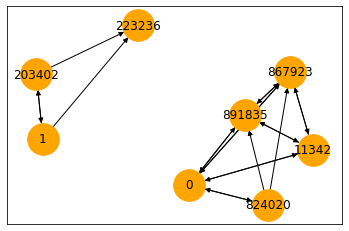
\includegraphics[width=0.5\textwidth]{img/DocPageRank_files/DocPageRank_20_0.png}
\end{center}

Remarque : Dans cet exemple il y a un \emph{dangling node} (223236). Un \emph{dandling node} \(q\) n'a de lien sortant vers aucun individu, et son ratio \(\frac{r^{i}(q)}{d(q)}\) vaut l'infini puisque \(d(q)=0\). Dans ce cas, on doit normalement fixer le ratio à \(0\) et rééquilibrer le poids des autres noeuds pour que la somme des rangs soit toujours égale à 1. Ici, pour simplifier les calculs et améliorer la vitesse de l'algorithme, nous retirons ce noeud.

\begin{Shaded}
\begin{Highlighting}[]
\NormalTok{dangling_nodes }\OperatorTok{=}\NormalTok{ [n }\ControlFlowTok{for}\NormalTok{ n }\KeywordTok{in}\NormalTok{ G1 }\ControlFlowTok{if}\NormalTok{ G1.out_degree(n, weight}\OperatorTok{=}\VariableTok{None}\NormalTok{) }\OperatorTok{==} \FloatTok{0.0}\NormalTok{] }
\BuiltInTok{print}\NormalTok{(dangling_nodes)}
\NormalTok{G1.remove_nodes_from(dangling_nodes) }\CommentTok{#car méthode ne gère pas dandling nodes}
\end{Highlighting}
\end{Shaded}

\begin{verbatim}
[223236]
\end{verbatim}

\begin{Shaded}
\begin{Highlighting}[]
\CommentTok{# Connexion au cluster / test en local}
\NormalTok{spark_conf }\OperatorTok{=}\NormalTok{ SparkConf()}\OperatorTok{\textbackslash{}}
\NormalTok{    .setAppName(}\StringTok{'Page Rank With PySpark'}\NormalTok{)}\OperatorTok{\textbackslash{}}
\NormalTok{    .setMaster(}\StringTok{'local'}\NormalTok{)}
\CommentTok{#sc.stop()}
\NormalTok{sc }\OperatorTok{=}\NormalTok{ SparkContext(conf}\OperatorTok{=}\NormalTok{spark_conf)}

\CommentTok{#Partitionner les données pour Spark}
\NormalTok{df }\OperatorTok{=}\NormalTok{ pd.read_csv(}\StringTok{"data/}\SpecialCharTok{\{\}\{\}}\StringTok{.txt"}\NormalTok{.}\BuiltInTok{format}\NormalTok{(fichier,nb_lignes),}
\NormalTok{                           sep}\OperatorTok{=}\StringTok{" "}\NormalTok{, names}\OperatorTok{=}\NormalTok{[}\StringTok{"in"}\NormalTok{,}\StringTok{"out"}\NormalTok{]) }
\NormalTok{df }\OperatorTok{=}\NormalTok{ df[df[}\StringTok{'in'}\NormalTok{]}\OperatorTok{!=}\NormalTok{dangling_nodes[}\DecValTok{0}\NormalTok{]]}
\NormalTok{df }\OperatorTok{=}\NormalTok{ df[df[}\StringTok{'out'}\NormalTok{]}\OperatorTok{!=}\NormalTok{dangling_nodes[}\DecValTok{0}\NormalTok{]]}
\NormalTok{df.to_csv(}\StringTok{"data/}\SpecialCharTok{\{\}\{\}}\StringTok{.txt"}\NormalTok{.}\BuiltInTok{format}\NormalTok{(fichier,nb_lignes), sep}\OperatorTok{=}\StringTok{" "}\NormalTok{,}
\NormalTok{          encoding}\OperatorTok{=}\StringTok{"utf-8"}\NormalTok{, index}\OperatorTok{=}\VariableTok{False}\NormalTok{, header}\OperatorTok{=}\VariableTok{None}\NormalTok{)}
\NormalTok{RddDataBase1 }\OperatorTok{=}\NormalTok{ sc.textFile(}\StringTok{"data/}\SpecialCharTok{\{\}\{\}}\StringTok{.txt"}\NormalTok{.}\BuiltInTok{format}\NormalTok{(fichier,nb_lignes))}
\end{Highlighting}
\end{Shaded}

\textbf{PageRank global}

\begin{Shaded}
\begin{Highlighting}[]
\BuiltInTok{print}\NormalTok{(}\StringTok{"Algorithme global en 2 itérations}\CharTok{\textbackslash{}n}\StringTok{"}\NormalTok{)}
\BuiltInTok{print}\NormalTok{(}\StringTok{"Pour alpha=1 : "}\NormalTok{)}
\NormalTok{afficher_resultats_PR(pagerank_global(G1, alpha}\OperatorTok{=}\DecValTok{1}\NormalTok{, max_iter}\OperatorTok{=}\DecValTok{2}\NormalTok{))}
\BuiltInTok{print}\NormalTok{(}\StringTok{"Pour alpha=0.85 :"}\NormalTok{)}
\NormalTok{afficher_resultats_PR(pagerank_global(G1, alpha}\OperatorTok{=}\FloatTok{0.85}\NormalTok{, max_iter}\OperatorTok{=}\DecValTok{2}\NormalTok{)) }
\end{Highlighting}
\end{Shaded}

\begin{verbatim}
Algorithme global en 2 itérations

Pour alpha=1 : 
Le temps de calcul est de 0.0004 secondes
La liste des noeuds et de leurs valeurs PageRank finales est
{0: 0.19, 11342: 0.131, 824020: 0.036, 867923: 0.179, 891835: 0.179, 1: 0.143, 203402: 0.143}


Pour alpha=0.85 :
Le temps de calcul est de 0.0002 secondes
La liste des noeuds et de leurs valeurs PageRank finales est
{0: 0.183, 11342: 0.133, 824020: 0.052, 867923: 0.173, 891835: 0.173, 1: 0.143, 203402: 0.143}
\end{verbatim}

L'algorithme global est ici très rapide à tourner en raison de la petite taille du graphe. Ce ne serait pas le cas pour un très gros graphe.

On remarque que le noeud 0 est celui qui présente le meilleur rang \emph{PageRank} (de nombreuses pages y font référence), suivi de près par les noeuds 867923 et 891835. En revanche, le noeud 824020 a un très mauvais score, ce qui s'explique facilement par le fait que seul le noeud 0 possède un hyperlien qui pointe vers lui.

\textbf{PageRank local non distribué}

\begin{Shaded}
\begin{Highlighting}[]
\BuiltInTok{print}\NormalTok{(}\StringTok{"Algorithme local en 2 itérations}\CharTok{\textbackslash{}n}\StringTok{"}\NormalTok{)}
\BuiltInTok{print}\NormalTok{(}\StringTok{"Pour alpha=1 : "}\NormalTok{)}
\NormalTok{afficher_resultats_PR(pagerank_local(G1, alpha}\OperatorTok{=}\DecValTok{1}\NormalTok{, max_iter}\OperatorTok{=}\DecValTok{2}\NormalTok{))}
\BuiltInTok{print}\NormalTok{(}\StringTok{"Pour alpha=0.85 :"}\NormalTok{)}
\NormalTok{afficher_resultats_PR(pagerank_local(G1, alpha}\OperatorTok{=}\FloatTok{0.85}\NormalTok{, max_iter}\OperatorTok{=}\DecValTok{2}\NormalTok{)) }
\end{Highlighting}
\end{Shaded}

\begin{verbatim}
Algorithme local en 2 itérations

Pour alpha=1 : 
Le temps de calcul est de 0.0004 secondes
La liste des noeuds et de leurs valeurs PageRank finales est
{0: 0.175, 11342: 0.167, 824020: 0.048, 867923: 0.163, 891835: 0.163, 1: 0.143, 203402: 0.143}


Pour alpha=0.85 :
Le temps de calcul est de 0.0001 secondes
La liste des noeuds et de leurs valeurs PageRank finales est
{0: 0.172, 11342: 0.159, 824020: 0.06, 867923: 0.162, 891835: 0.162, 1: 0.143, 203402: 0.143}
\end{verbatim}

L'approximation locale de \emph{PageRank} est encore plus rapide à tourner que la résolution globale de l'algorithme.

Bien que les résultats soient différents (c'est normal, l'algorithme l'est aussi !). Les résultats vont dans le même sens que l'implémentation précédente. Le noeud 0 présente toujours le meilleur \emph{PageRank} et le noeud 824020 toujours le moins bon.

\textbf{PageRank local distribué}

\begin{Shaded}
\begin{Highlighting}[]
\BuiltInTok{print}\NormalTok{(}\StringTok{"Algorithme local en 2 itérations}\CharTok{\textbackslash{}n}\StringTok{"}\NormalTok{)}
\BuiltInTok{print}\NormalTok{(}\StringTok{"Pour alpha=1 : "}\NormalTok{)}
\NormalTok{afficher_resultats_PR(pagerank_local_spark(RddDataBase1, alpha}\OperatorTok{=}\DecValTok{1}\NormalTok{, max_iter}\OperatorTok{=}\DecValTok{2}\NormalTok{))}
\BuiltInTok{print}\NormalTok{(}\StringTok{"Pour alpha=0.85 :"}\NormalTok{)}
\NormalTok{afficher_resultats_PR(pagerank_local_spark(RddDataBase1, alpha}\OperatorTok{=}\FloatTok{0.85}\NormalTok{, max_iter}\OperatorTok{=}\DecValTok{2}\NormalTok{)) }
\end{Highlighting}
\end{Shaded}

\begin{verbatim}
Algorithme local en 2 itérations

Pour alpha=1 : 
Le temps de calcul est de 0.1126 secondes
La liste des noeuds et de leurs valeurs PageRank finales est
{0: 0.175, 1: 0.143, 11342: 0.167, 203402: 0.143, 824020: 0.048, 867923: 0.163, 891835: 0.163}


Pour alpha=0.85 :
Le temps de calcul est de 0.1132 secondes
La liste des noeuds et de leurs valeurs PageRank finales est
{0: 0.172, 1: 0.143, 11342: 0.159, 203402: 0.143, 824020: 0.06, 867923: 0.162, 891835:     0.162}
\end{verbatim}

Enfin, les résultats de l'algorithme précédent implémenté en utilisant des calculs distribués (\emph{framework} Spark) présente les mêmes résultats (l'algorithme est identique et est simplement parallélisé).

Il met beaucoup plus de temps que l'algorithme non distribué à tourner, mais il ne faut pas s'arrêter sur ce résultat. En effet, ici la taille du graphe est très petite. La partie suivante va montrer que pour des graphes plus grands et un nombre d'itérations plus important, l'efficacité de l'algorithme parallélisé va s'avérer bien meilleure que celle de l'algorithme initial.

\hypertarget{graphiques-de-mesure-de-performance}{%
\subsection{Graphiques de mesure de performance}\label{graphiques-de-mesure-de-performance}}

Cette dernière partie vise à illustrer l'efficacité du calcul distribué avec Spark par rapport à la version de l'algorithme sans calcul distribué.

\begin{Shaded}
\begin{Highlighting}[]
\NormalTok{spark_conf }\OperatorTok{=}\NormalTok{ SparkConf()}\OperatorTok{\textbackslash{}}
\NormalTok{    .setAppName(}\StringTok{'Page Rank With PySpark'}\NormalTok{)}\OperatorTok{\textbackslash{}}
\NormalTok{    .setMaster(}\StringTok{'local'}\NormalTok{)}
\NormalTok{sc.stop()}
\NormalTok{sc }\OperatorTok{=}\NormalTok{ SparkContext(conf}\OperatorTok{=}\NormalTok{spark_conf)}
\end{Highlighting}
\end{Shaded}

\hypertarget{temps-de-calcul-en-fonction-de-la-taille-du-graphe-uxe0-nombre-dituxe9rations-fixuxe9}{%
\subsubsection{Temps de calcul en fonction de la taille du graphe (à nombre d'itérations fixé)}\label{temps-de-calcul-en-fonction-de-la-taille-du-graphe-uxe0-nombre-dituxe9rations-fixuxe9}}

Conformément aux intuitions, plus la taille du graphe augmente, plus Spark présente des avantages en termes de temps de calcul. En effet, quand la taille du fichier est très petite, le calcul distribué opéré par Spark ne présente pas d'avantage voire détériore le temps de calcul par rapport à la version non distribuée. En revanche, on remarque qu'à partir d'une certaine taille de graphe, l'efficacité de Spark devient explosive, si bien que nous avons choisi de représenter l'axe des abscisse sous forme logarithmique.

Nous observons la même conclusion, pour 5 et 20 itérations (avec bien sûr, des niveaux de temps de calcul, en ordonnée, différents). C'est pourquoi nous regardons d'un peu plus près l'évolution du temps de calcul en fonction du nombre d'itérations dans la partie suivante.

\begin{Shaded}
\begin{Highlighting}[]
\NormalTok{nbs_lignes}\OperatorTok{=}\NormalTok{[}\DecValTok{100}\NormalTok{,}\DecValTok{1000}\NormalTok{,}\DecValTok{10000}\NormalTok{,}\DecValTok{100000}\NormalTok{,}\DecValTok{1000000}\NormalTok{,}\DecValTok{10000000}\NormalTok{]}
\NormalTok{with_spark_list, without_spark_list }\OperatorTok{=}\NormalTok{ creer_donnees_graphique_timer_lignes(}
\NormalTok{    nbs_lignes,}
\NormalTok{    nb_iter}\OperatorTok{=}\DecValTok{5}\NormalTok{)}
\NormalTok{creer_graphique_timer_lignes(nbs_lignes,with_spark_list,without_spark_list,nb_iter}\OperatorTok{=}\DecValTok{5}\NormalTok{)}
\end{Highlighting}
\end{Shaded}

\begin{center}
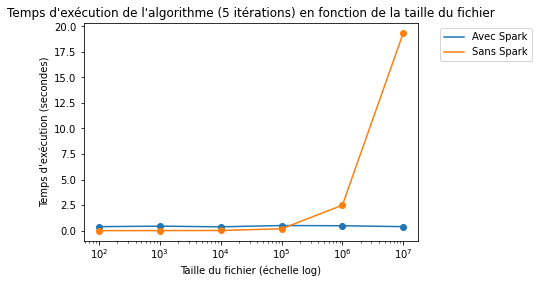
\includegraphics[width=0.7\textwidth]{img/DocPageRank_files/DocPageRank_36_0.png}
\end{center}

\begin{Shaded}
\begin{Highlighting}[]
\NormalTok{nbs_lignes}\OperatorTok{=}\NormalTok{[}\DecValTok{100}\NormalTok{,}\DecValTok{1000}\NormalTok{,}\DecValTok{10000}\NormalTok{,}\DecValTok{100000}\NormalTok{,}\DecValTok{1000000}\NormalTok{,}\DecValTok{10000000}\NormalTok{]}
\NormalTok{with_spark_list, without_spark_list }\OperatorTok{=}\NormalTok{ creer_donnees_graphique_timer_lignes(}
\NormalTok{    nbs_lignes,}
\NormalTok{    nb_iter}\OperatorTok{=}\DecValTok{20}\NormalTok{)}
\NormalTok{creer_graphique_timer_lignes(nbs_lignes,with_spark_list,}
\NormalTok{                             without_spark_list,nb_iter}\OperatorTok{=}\DecValTok{20}\NormalTok{)}
\end{Highlighting}
\end{Shaded}

\begin{center}
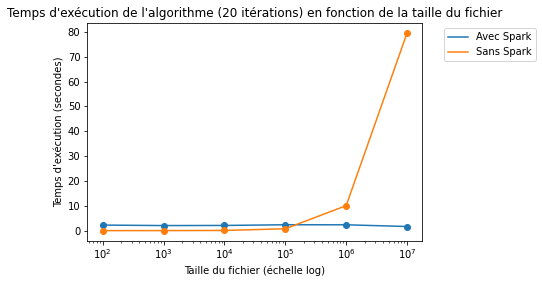
\includegraphics[width=0.7\textwidth]{img/DocPageRank_files/DocPageRank_37_0.png}
\end{center}

\hypertarget{temps-de-calcul-en-fonction-du-nombre-dituxe9rations-uxe0-taille-de-graphe-fixuxe9e}{%
\subsubsection{Temps de calcul en fonction du nombre d'itérations (à taille de graphe fixée)}\label{temps-de-calcul-en-fonction-du-nombre-dituxe9rations-uxe0-taille-de-graphe-fixuxe9e}}

En plus d'être de plus en plus efficace au fur et à mesure que la taille des graphes augmente, Spark est également de plus en plus efficace au fur et à mesure que le nombre d'itérations augmente.

\begin{Shaded}
\begin{Highlighting}[]
\NormalTok{nbs_iters}\OperatorTok{=}\NormalTok{[}\DecValTok{10}\NormalTok{,}\DecValTok{100}\NormalTok{,}\DecValTok{1000}\NormalTok{]}
\NormalTok{with_spark_list, without_spark_list }\OperatorTok{=}\NormalTok{ creer_donnees_graphique_timer_iters(}
\NormalTok{    nbs_iters,nb_lignes}\OperatorTok{=}\DecValTok{1000000}\NormalTok{)}
\NormalTok{creer_graphique_timer_iters(nbs_iters,with_spark_list,}
\NormalTok{                            without_spark_list,nb_lignes}\OperatorTok{=}\DecValTok{1000000}\NormalTok{)}
\end{Highlighting}
\end{Shaded}

\begin{center}
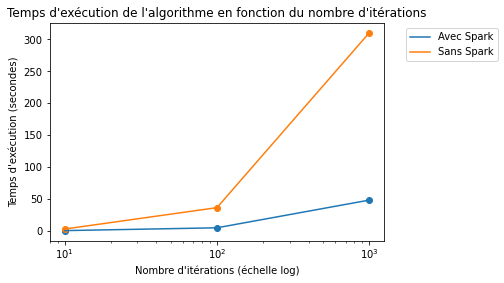
\includegraphics[width=0.7\textwidth]{img/DocPageRank_files/DocPageRank_39_0.png}
\end{center}

\textbf{Pour conclure}, la distribution des calculs de l'algorithme \emph{PageRank} fait gagner un temps considérable à partir d'une certaine taille de graphe et quand le nombre d'itérations de l'algorithme est suffisamment important.

\hypertarget{ouvertures}{%
\section{Ouvertures}\label{ouvertures}}

\hypertarget{spark-un-outil-pas-totalement-magique}{%
\subsection{Spark, un outil pas totalement magique}\label{spark-un-outil-pas-totalement-magique}}

Ce travail a montré que Spark est une méthode assez intuitive et visiblement particulièrement efficace pour distribuer l'algorithme de \emph{PageRank} (boucle d'étapes Map-Reduce) sur des graphes de grandes tailles (\emph{Big Data}).

Toutefois, il existe des cas où l'usage de Spark peut devenir inefficace. En effet, comme son fonctionnement est très sophistiqué, cela amène à des tâches d'initialisation chronophages. C'est pourquoi il est en pratique important de monitorer la durée d'initialisation et de la comparer avec la durée computationnelle.

On le voit d'ailleurs sur nos données, la durée d'initialisation de l'algorithme \emph{PageRank} est sensiblement plus importante dans la version distribuée utilisant Spark. Cet écart d'initialisation est d'autant plus grand que la taille du graphe est grande.

\begin{Shaded}
\begin{Highlighting}[]
\NormalTok{nbs_lignes}\OperatorTok{=}\NormalTok{[}\DecValTok{100}\NormalTok{,}\DecValTok{1000}\NormalTok{,}\DecValTok{10000}\NormalTok{,}\DecValTok{100000}\NormalTok{,}\DecValTok{1000000}\NormalTok{,}\DecValTok{10000000}\NormalTok{]}
\NormalTok{with_spark_list, without_spark_list }\OperatorTok{=}\NormalTok{ creer_donnees_graphique_timer_lignes(}
\NormalTok{    nbs_lignes,nb_iter}\OperatorTok{=}\DecValTok{5}\NormalTok{, timer_mapreduce}\OperatorTok{=}\VariableTok{False}\NormalTok{)}
\NormalTok{creer_graphique_timer_lignes(nbs_lignes,with_spark_list,}
\NormalTok{                             without_spark_list,nb_iter}\OperatorTok{=}\DecValTok{5}\NormalTok{,timer_mapreduce}\OperatorTok{=}\VariableTok{False}\NormalTok{)}
\end{Highlighting}
\end{Shaded}

\begin{center}
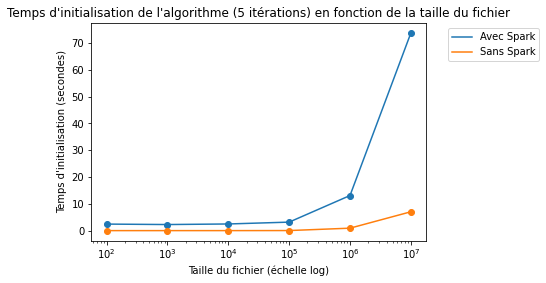
\includegraphics[width=0.7\textwidth]{img/DocPageRank_files/DocPageRank_43_0.png}
\end{center}

\hypertarget{spark-en-cluster}{%
\subsection{Spark en Cluster}\label{spark-en-cluster}}

Nous avions utilisé jusqu'à présent l'installation de Spark en local. Dans ce mode de déploiement, Spark exécute tout dans une unique machine virtuelle Java (JVM).

Cette installation n'est pas strictement identique à celle dans un cluster réel. Dans un ``vrai'' cluster, il faut penser à uploader les données et ne pas les conserver uniquement en local. Il faut également installer sur chaque machine du cluster les dépendances du script, dès la création du cluster ou avant de lancer un script pour les installations plus spécifiques. Il est aussi plus complexe de débugger le code (par exemple, la fonction \texttt{print} peut ne pas fonctionner sur les clusters).

Pour nous initier à l'utilisation de cluster, nous avons créé un environnement dans lequel nous avons créé une machine maître (\emph{master}) et plusieurs machines secondaires (\emph{workers}). Pour cela, nous avons utilisé les commandes suivantes dans notre terminal windows.

\begin{verbatim}
# Attention code à exécuter en mode administrateur !
# Créer un noeud maître
cd "C:/Users/Spark/spark-3.0.1-bin-hadoop2.7/bin"
spark-class org.apache.spark.deploy.master.Master
# Créer autant de noeuds "workers" que souhaité (répéter la commande qui suit)
cd "C:/Users/Spark/spark-3.0.1-bin-hadoop2.7/bin"
spark-class org.apache.spark.deploy.worker.Worker spark://192.168.1.10:7077
\end{verbatim}

Suite à ces instructions, nous pouvons consulter à l'adresse \url{http://192.168.1.10:8080/} les différents noeuds souhaités. La figure \ref{fig:fig3} montre un exemple avec 1 \emph{master} et 2 \emph{workers}.

\begin{figure}
\begin{center}
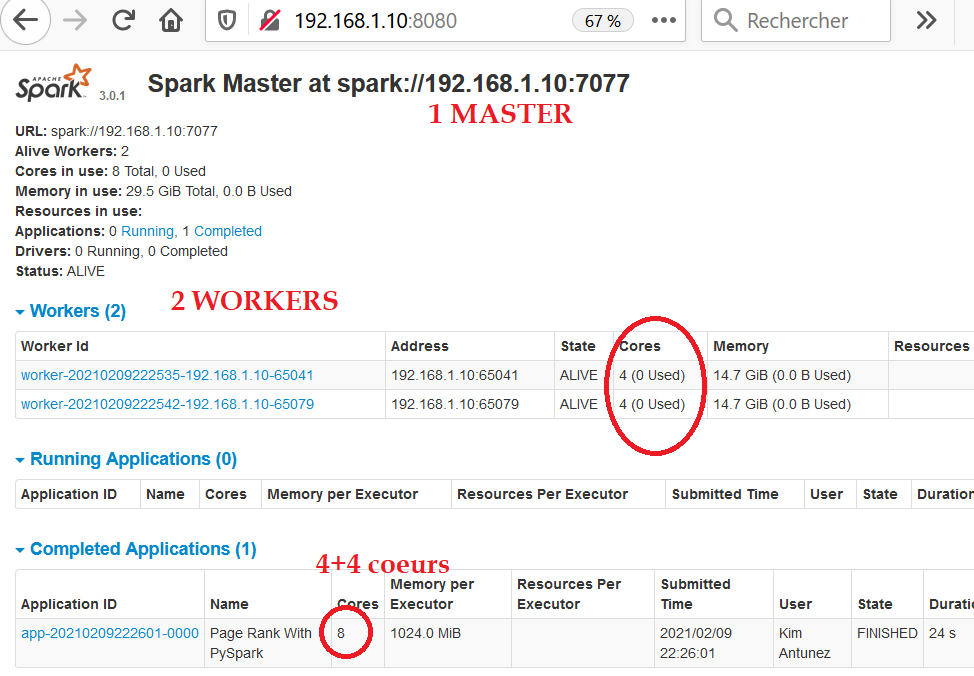
\includegraphics[width=0.8\textwidth]{img/spark.png}
\end{center}
\captionsetup{margin=0cm,format=hang,justification=justified}
\caption{Un aperçu de Spark}\label{fig:fig3}
\end{figure}

Nous avons ensuite évalué le temps de calcul de l'algorithme \emph{PageRank} (\texttt{nb\_lignes} = 10000, \texttt{alpha}= 0,85 et \texttt{max\_iter} = 200) en fonction de différentes tailles de clusters.

\begin{longtable}[]{@{}ll@{}}
\toprule
\textbf{nombre de workers} & \textbf{temps de calcul (sec)}\tabularnewline
\midrule
\endhead
aucun (local) & 16,80\tabularnewline
1 & 10,15\tabularnewline
2 & 10,59\tabularnewline
3 & 11,45\tabularnewline
4 & 10,25\tabularnewline
5 & 13,22\tabularnewline
11 & 09,93\tabularnewline
\bottomrule
\end{longtable}

Les résultats sont assez étonnants et difficiles à interpréter\ldots{} Il aurait peut-être fallu effectuer plusieurs fois les calculs et en faire la moyenne pour avoir des données fiables et interprétables. Mais nous pouvons voir que l'ajout de machines secondaires (\emph{workers}) améliore globalement la vitesse de l'algorithme par rapport à la version paramétrée en local.

\newpage

\begin{Shaded}
\begin{Highlighting}[]
\CommentTok{# Connexion au cluster créé dans le terminal}
\NormalTok{fichier }\OperatorTok{=} \StringTok{"web-Google"}
\NormalTok{nb_lignes}\OperatorTok{=}\DecValTok{10000}
\NormalTok{spark_conf }\OperatorTok{=}\NormalTok{ SparkConf()}\OperatorTok{\textbackslash{}}
\NormalTok{    .setAppName(}\StringTok{'Page Rank With PySpark'}\NormalTok{)}\OperatorTok{\textbackslash{}}
\NormalTok{    .setMaster(}\StringTok{'spark://192.168.1.10:7077'}\NormalTok{) }\CommentTok{#local}
\NormalTok{sc.stop()}
\NormalTok{sc }\OperatorTok{=}\NormalTok{ SparkContext(conf}\OperatorTok{=}\NormalTok{spark_conf)}

\CommentTok{#Partitionner les données pour Spark}
\NormalTok{RddDataBase1 }\OperatorTok{=}\NormalTok{ sc.textFile(}\StringTok{"data/}\SpecialCharTok{\{\}\{\}}\StringTok{.txt"}\NormalTok{.}\BuiltInTok{format}\NormalTok{(fichier,nb_lignes))}
\end{Highlighting}
\end{Shaded}

\begin{Shaded}
\begin{Highlighting}[]
\CommentTok{# local}
\NormalTok{pagerank_local_spark(RddDataBase1, alpha}\OperatorTok{=}\FloatTok{0.85}\NormalTok{, max_iter}\OperatorTok{=}\DecValTok{200}\NormalTok{,}
\NormalTok{                     timer_mapreduce}\OperatorTok{=}\VariableTok{True}\NormalTok{, only_timer}\OperatorTok{=}\VariableTok{True}\NormalTok{)}
\end{Highlighting}
\end{Shaded}

\begin{verbatim}
16.797327700000096
\end{verbatim}

\begin{Shaded}
\begin{Highlighting}[]
\CommentTok{# un worker}
\NormalTok{pagerank_local_spark(RddDataBase1, alpha}\OperatorTok{=}\FloatTok{0.85}\NormalTok{, max_iter}\OperatorTok{=}\DecValTok{200}\NormalTok{,}
\NormalTok{                     timer_mapreduce}\OperatorTok{=}\VariableTok{True}\NormalTok{, only_timer}\OperatorTok{=}\VariableTok{True}\NormalTok{)}
\end{Highlighting}
\end{Shaded}

\begin{verbatim}
10.153115699999944
\end{verbatim}

\begin{Shaded}
\begin{Highlighting}[]
\CommentTok{# deux workers}
\NormalTok{pagerank_local_spark(RddDataBase1, alpha}\OperatorTok{=}\FloatTok{0.85}\NormalTok{, max_iter}\OperatorTok{=}\DecValTok{200}\NormalTok{,}
\NormalTok{                     timer_mapreduce}\OperatorTok{=}\VariableTok{True}\NormalTok{, only_timer}\OperatorTok{=}\VariableTok{True}\NormalTok{)}
\end{Highlighting}
\end{Shaded}

\begin{verbatim}
10.588963599999943
\end{verbatim}

\begin{Shaded}
\begin{Highlighting}[]
\CommentTok{# trois workers}
\NormalTok{pagerank_local_spark(RddDataBase1, alpha}\OperatorTok{=}\FloatTok{0.85}\NormalTok{, max_iter}\OperatorTok{=}\DecValTok{200}\NormalTok{,}
\NormalTok{                     timer_mapreduce}\OperatorTok{=}\VariableTok{True}\NormalTok{, only_timer}\OperatorTok{=}\VariableTok{True}\NormalTok{)}
\end{Highlighting}
\end{Shaded}

\begin{verbatim}
11.451345600000195
\end{verbatim}

\begin{Shaded}
\begin{Highlighting}[]
\CommentTok{# quatre workers}
\NormalTok{pagerank_local_spark(RddDataBase1, alpha}\OperatorTok{=}\FloatTok{0.85}\NormalTok{, max_iter}\OperatorTok{=}\DecValTok{200}\NormalTok{,}
\NormalTok{                     timer_mapreduce}\OperatorTok{=}\VariableTok{True}\NormalTok{, only_timer}\OperatorTok{=}\VariableTok{True}\NormalTok{)}
\end{Highlighting}
\end{Shaded}

\begin{verbatim}
10.250091500000053
\end{verbatim}

\begin{Shaded}
\begin{Highlighting}[]
\CommentTok{# cinq workers}
\NormalTok{pagerank_local_spark(RddDataBase1, alpha}\OperatorTok{=}\FloatTok{0.85}\NormalTok{, max_iter}\OperatorTok{=}\DecValTok{200}\NormalTok{,}
\NormalTok{                     timer_mapreduce}\OperatorTok{=}\VariableTok{True}\NormalTok{, only_timer}\OperatorTok{=}\VariableTok{True}\NormalTok{)}
\end{Highlighting}
\end{Shaded}

\begin{verbatim}
13.222826199999872
\end{verbatim}

\begin{Shaded}
\begin{Highlighting}[]
\CommentTok{# onze workers}
\NormalTok{pagerank_local_spark(RddDataBase1, alpha}\OperatorTok{=}\FloatTok{0.85}\NormalTok{, max_iter}\OperatorTok{=}\DecValTok{200}\NormalTok{,}
\NormalTok{                     timer_mapreduce}\OperatorTok{=}\VariableTok{True}\NormalTok{, only_timer}\OperatorTok{=}\VariableTok{True}\NormalTok{)}
\end{Highlighting}
\end{Shaded}

\begin{verbatim}
9.9428640000001
\end{verbatim}

\nocite{*}

\begin{thebibliography}{999}
\bibitem[Brin, Page (1998)]{Brin} Brin, S., \& Page, L. (1998). The anatomy of a large-scale hypertextual web search engine. Computer networks and ISDN systems, 30(1-7), 107-117.
\bibitem[Chen \emph{et al.} (2004)]{Chen} Chen, Y. Y., Gan, Q., \& Suel, T. (2004). Local methods for estimating pagerank values. In Proceedings of the thirteenth ACM international conference on Information and knowledge management (pp. 381-389).
\bibitem[Chen, Dyer (2010)]{Lin} Lin, J., \& Dyer, C. (2010). Data-intensive text processing with MapReduce. Synthesis Lectures on Human Language Technologies, 3(1), 1-177.
\end{thebibliography}

\url{http://www.economiematin.fr/news-algorythme-page-rank-popularite-web}

\url{https://www.geeksforgeeks.org/page-rank-algorithm-implementation/}

\url{http://www.bibmath.net/dico/index.php?action=affiche&quoi=./p/perron-frobenius.html}

\url{https://univalence.io/blog/articles/shuffle-dans-spark-reducebykey-vs-groupbykey/}

\end{document}
